\subsection{Generalized Coordinates}
\label{subsect:application-generalized-coordinates}

\begin{frame}
  \frametitle{\insertsubsection}
  \begin{itemize}
    \item Generalized coordinates \begin{itemize}
      \item \makebox[.5cm]{\hfill$x \colon$}\makebox[.9cm]{\hfill$V_\text{u}(\Pi)$} ${\to \mathbb{R}}$
      \item \makebox[.5cm]{\hfill$y \colon$}\makebox[.9cm]{\hfill$V_\text{u}(\Pi)$} ${\to \mathbb{R}}$
      \item \makebox[.5cm]{\hfill$\varphi \colon$}\makebox[.9cm]{\hfill$\Pi\phantom{)}$} ${\to (-180 \degrees, 180 \degrees)}$
      \item \makebox[.5cm]{\hfill$p \colon$}\makebox[.9cm]{\hfill$V_\text{c}(\Pi)$} ${\to (0, 1)}$
    \end{itemize}
  \end{itemize}
  \begin{figure}
    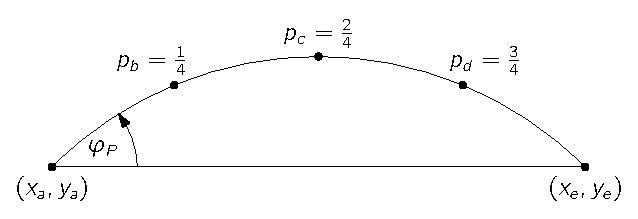
\includegraphics[height=2.0cm]{Resources/Generalized-Coordinates-Example.eps}
    \caption{Generalized coordinates for a single path ${P = abcde}$ with equi-length edges.}
  \end{figure}
\end{frame}

\begin{frame}[c]
  \frametitle{\insertsubsection}
  \begin{algorithm}[H]
    \caption{Transformation to Cartesian coordinates ${\vec{r}(v)}$}
    \SetKwData{CircularArc}{CircularArc}
    \SetKwData{PointForProgress}{pointForProgress}
    \ForEach{${v \in V_\text{u}(\Pi)}$}{
      ${\vec{r}(v) \gets (x({v}), y({v}))}$\;
    }
    \;
    \ForEach{${P = (v_1, \ldots, v_n) \in \Pi}$}{
      ${\Gamma(P) \gets \CircularArc(\vec{r}(v_1), \vec{r}(v_n), \varphi(P))}$\;
      \;
      \ForEach{${v \in (v_2, \ldots, v_{n-1})}$}{
        ${\vec{r}(v) \gets \Gamma(P).\PointForProgress(p(v))}$\;
      }
    }
    \;
  \end{algorithm}
\end{frame}
